\section{Results}\label{sec-results}

This section is divided into three main topics. First, we will discuss
the social media platforms and languages students use, along with the
objectives they pursue when making videos. Second, we will describe what
students do before and after making videos. Third, we will examine
students' perceptions of language learning through video-making.

\subsection{Social media platforms, languages, and objectives}\label{sub-sec-socialmediaplatforms}

In general, 46 people, or only 21.7\% of the participants of the overall
questionnaire, reported that they occasionally had been making videos in
a broad sense (including reels and stories on Instagram). We will centre
most of our results section on these participants.

Stories on Instagram and videos on YouTube were the most frequently
produced types of videos according to \Cref{fig-01}. Instagram stories are
used 28.3\% \emph{sometimes} and 13\% \emph{frequently}, meanwhile,
videos on YouTube are made 34.8\% \emph{sometimes} and 8.7\%
\emph{frequently}. Notably, almost nobody used Twitch and a small
percentage of the students made videos on TikTok (15.2\%).

\begin{figure}[htbp]
\centering
\begin{minipage}{\textwidth}
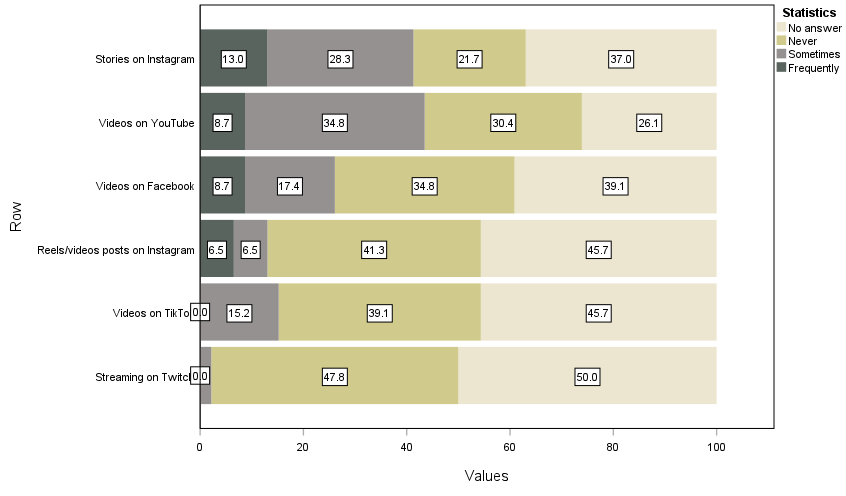
\includegraphics[width=\textwidth]{Fig-1.png}
\caption{Frequency of production of different types of videos.}
\label{fig-01}
\source{Own elaboration.}
\end{minipage}
\end{figure}

We also observe a pattern across all platforms, with the least common
response being to make videos frequently (from 13\% on Instagram to 0\%
on TikTok), indicating that a relatively low percentage of respondents
makes videos frequently, especially in comparison with the practice of
watching videos \cite{shafirova2023}. Moreover, we found a
correlation between the age of the students and the types of video
production. The correlation was found in the social media platforms of
TikTok, YouTube and Facebook, in which older students (older than 36)
tend to make videos for Facebook (due to cross tabulation with Pearson
chi-square test with 0.019 significance in case of YouTube and 0.004 in
case of Facebook). Meanwhile, younger students (from 18 to 23) tend to
make videos on TikTok (due to cross tabulation with Pearson chi-square
test with 0.008 significance). It is noteworthy that, on Instagram, we
did not find any correlation with age.

In general, in our data, age does not influence the frequency of making
videos, however, it points out that some social media platforms are more
frequently used by younger respondents and some by slightly older
respondents (similarly found in the dataset concerning the US population
from \textcite{ortizo-spina2019}). Moreover, the students post videos in
different languages, mostly in Portuguese and English (\Cref{tab-04}), while
other languages have a relatively smaller presence (max. 20\% with
Spanish on Facebook).

\begin{table}[htbp]
\centering
\begin{threeparttable}
\caption{Languages and platforms of video production: multiple choice response.}
\label{tab-04}
\begin{tabular}{*{11}{l}}
\toprule
Platforms & \multicolumn{2}{c}{YouTube} & \multicolumn{2}{c}{Facebook} &  \multicolumn{2}{c}{Instagram} & \multicolumn{2}{c}{TikTok} & \multicolumn{2}{c}{Twitch} \\
\midrule
Portuguese & 22 & 88\% & 13 & 86.7\% & 19 & 95\% & 5 & 71.4\% & 0 & 0\% \\
English    & 13 & 52\% & 6  & 40\%   & 9  & 45\% & 5 & 71.4\% & 1 & 50\% \\
Spanish    & 3  & 12\% & 3  & 20\%   & 1  & 5\%  & 0 & 0\%    & 0 & 0\% \\
Italian    & 2  & 8\%  & 2  & 13.3\% & 1  & 5\%  & 0 & 0\%    & 0 & 0\% \\
French     & 1  & 4\%  & 2  & 13.3\% & 0  & 0\%  & 0 & 0\%    & 0 & 0\% \\
Crioulo    & 0  & 0\%  & 0  & 0\%    & 1  & 5\%  & 0 & 0\%    & 0 & 0\% \\
Persian    & 0  & 0\%  & 1  & 6.7\%  & 0  & 0\%  & 0 & 0\%    & 0 & 0\% \\
Other      & 2  & 8\%  & 1  & 6.7\%  & 1  & 5\%  & 2 & 28.6\% & 1 & 50\% \\
\rule{0pt}{3ex}%
Total & 44 & 176\% & 28 & 186.7\% & 32 & 160\% & 12 & 171.4\% & 2 & 100\% \\
\bottomrule
\end{tabular}
\source{Own elaboration.}
\end{threeparttable}
\end{table}




In comparison, our previous study shows that video consumption on social
media and streaming platforms could be considered more diverse and
plurilingual. Even though English and Portuguese were still the most
popular languages, Spanish was used by roughly half of the participants
on streaming platforms such as Netflix and HBO. Additionally, such
languages as French, Italian, Korean or Japanese were also present, with
more than 10\% on various platforms \cite{shafirova2023}. There
could be various reasons for this difference in language variety in
video production and consumption. One possible explanation could be the
amount of resources available for watching videos in languages you do
not have a perfect command of, such as subtitles in different languages,
captions, scripts and more \cite{shafirova2023}.

Moreover, we asked the participants if they tended to use several
languages in one video. The participants responded with 26.1\% ``yes'',
with the main objective of reaching out to a vast audience (41.6\%), or
because of being multilingual (30\%).

\subsection{Why students make and post videos}

To understand students' intentions behind video production, we asked
about their objectives when making videos. According to \Cref{fig-02}, the
majority of the students make videos to ``have fun'' (63\%), which goes
along with previous research on video creation beyond the classroom
\cite{zhang2022}.

\begin{figure}[htbp]
\centering
\begin{minipage}{\textwidth}
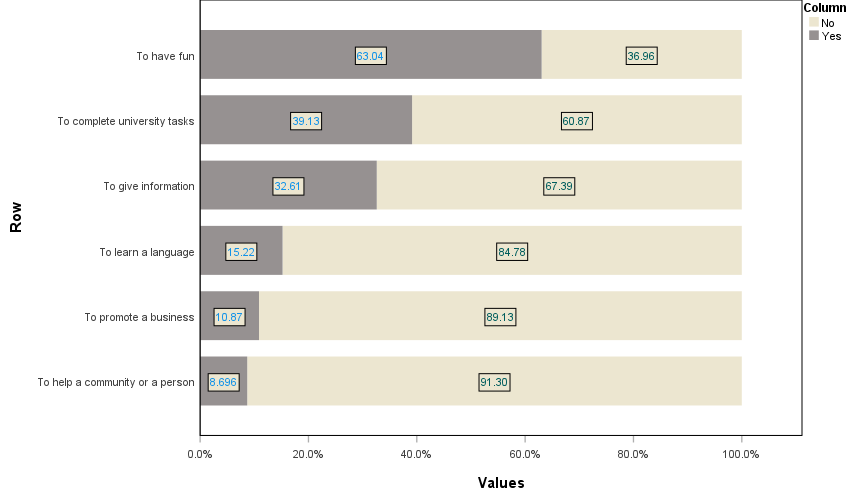
\includegraphics[width=\textwidth]{Fig-2.png}
\source{Own elaboration.}
\caption{Objectives to make videos.}
\label{fig-02}
\end{minipage}
\end{figure}

However, the second most popular answer is ``to complete university
tasks'' (39.1\%), which is a thought-provoking result indicating that
some of the university tasks require students to make videos (similar
results at the school level in \textcite{cassany2021}). It would be
valuable to explore the potential differences between the videos created
for leisure and those made as university tasks, even though these videos
would not necessarily be connected to language learning.

Moreover, the third answer was ``to give information'' (33\%), which
also seems like a serious and not entertaining goal, which can include
making videos or reposts of some news or events. This goes against the
assumption of some researchers that social media is always used only for
entertainment purposes \textcite{rosyida2019}. Also, the option ``to
learn a language'' was not popular (15.2\%), which is an expected result
as only 33\% of the participants are current language learners.

\subsection{What students do before and after producing videos}

Much like when watching videos online \cite{shafirova2023},
around half of the respondents were engaged in some communicative
actions before and after making a video. According to \Cref{tab-05} and \Cref{tab-06},
the communicative actions included searching (information or visuals),
reading (comments), writing (descriptions of the videos), watching
videos (to analyse similar videos), translating and interacting with
others (collaborating with others, responding to comments, making video
responses). The most frequent action before video production is
searching for information (\Cref{tab-05}), while the most frequent after
production is reading the comments or feedback on the videos (\Cref{tab-06}).
The options of writing descriptions or interacting with others were less
popular (roughly half of the responses).


\begin{table}[htbp]
\centering
\small
\begin{threeparttable}
\caption{Communicative actions made before video production.}
\label{tab-05}
\begin{tabular}{*{13}{l}}
\toprule
\multicolumn{1}{{>{\raggedright\arraybackslash}p{0.11\textwidth}}}{Actions} &
\multicolumn{2}{{>{\raggedright\arraybackslash}p{0.11\textwidth}}}{Search for information} &
\multicolumn{2}{{>{\raggedright\arraybackslash}p{0.11\textwidth}}}{Search for visual aid} &
\multicolumn{2}{{>{\raggedright\arraybackslash}p{0.11\textwidth}}}{Analyse similar videos} &
\multicolumn{2}{{>{\raggedright\arraybackslash}p{0.11\textwidth}}}{Write short descriptions} &
\multicolumn{2}{{>{\raggedright\arraybackslash}p{0.11\textwidth}}}{Collaborate with others} &
\multicolumn{2}{{>{\raggedright\arraybackslash}p{0.11\textwidth}}}{Make translations} \\
\midrule
Languages & N & \% & N & \% & N & \% & N & \% & N & \% & N & \% \\ 
Portuguese & 16 & 69.6\% & 11 & 47.8\% & 10 & 43.5\% & 11 & 47.8\% & 9  & 39.1\% & 7  & 30.4\% \\ 
English    & 18 & 78.3\% & 15 & 65.2\% & 11 & 47.8\% & 7  & 30.4\% & 7  & 30.4\% & 9  & 39.1\% \\ 
Spanish    & 3  & 13\%   & 2  & 8.7\%  & 3  & 13\%   & 1  & 4.3\%  & 2  & 8.7\%  & 1  & 4.3\%  \\ 
Italian    & 2  & 8.7\%  & 2  & 8.7\%  & 2  & 8.7\%  & 1  & 4.3\%  & 2  & 8.7\%  & 1  & 4.3\%  \\ 
French     & 2  & 8.7\%  & 2  & 8.7\%  & 2  & 8.7\%  & 0  & 0\%    & 2  & 8.7\%  & 1  & 4.3\%  \\ 
Chinese    & 1  & 4.3\%  & 1  & 4.3\%  & 0  & 0\%    & 1  & 4.3\%  & 0  & 0\%    & 0  & 0\%    \\ 
Persian    & 1  & 4.3\%  & 0  & 0\%    & 0  & 0\%    & 0  & 0\%    & 0  & 0\%    & 0  & 0\%    \\ 
Other      & 1  & 4.3\%  & 0  & 0\%    & 0  & 0\%    & 0  & 0\%    & 0  & 0\%    & 0  & 0\%    \\ 
\rule{0pt}{3ex}%
Total     & 44 & 191.2\% & 33 & 143.4\% & 28 & 121.7\% & 21 & 91.1\% & 22 & 95.6\% & 19 & 82.4\% \\ 
\bottomrule
\end{tabular}
\source{Own elaboration.}
\end{threeparttable}
\end{table}

Interestingly, if videos were mostly created in Portuguese and English,
the actions made before and after video production had more linguistic
variability, with the 7 languages present before video production, and
11 after production.

Furthermore, we made a comparison or cross-tabulation comparing the
participants\textquotesingle{} mother tongues with the actions taken
before video production (\Cref{tab-05}). The results showed that most
participants were using a foreign language before and after making a
video. In the case of activities made before video production, several
participants used such foreign languages as English, French and Italian.
Also, some participants used their mother tongues, including Portuguese,
Spanish, Chinese and Persian. Similar data emerged when comparing the
responses concerning the actions taken after posting the videos in
relation to the participants' mother tongues (\Cref{tab-06}).


\begin{table}[htbp]
\centering
\begin{threeparttable}
\caption{Communicative actions made after video production.}
\label{tab-06}
\begin{tabular}{*{7}{l}}
\toprule
Actions &
\multicolumn{2}{{{>{\raggedright\arraybackslash}p{0.25\textwidth}}}}{Read comments, chat, reactions} &
\multicolumn{2}{{>{\raggedright\arraybackslash}p{0.14285714285\textwidth}}}{Respond to the comments} &
\multicolumn{2}{{>{\raggedright\arraybackslash}p{0.14285714285\textwidth}}}{Make video responses to comments} \\
\midrule
Portuguese & 19 & 79.2\% & 8 & 33.3\% & 3 & 12.5\% \\ 
English    & 17 & 70.8\% & 9 & 37.5\% & 3 & 12.5\% \\ 
Spanish    & 7  & 29.2\% & 3 & 12.5\% & 1 & 4.2\%  \\ 
Italian    & 5  & 20.8\% & 3 & 12.5\% & 1 & 4.2\%  \\ 
French     & 5  & 20.8\% & 2 & 8.3\%  & 2 & 8.3\%  \\ 
Chinese    & 2  & 8.3\%  & 1 & 4.2\%  & 1 & 4.2\%  \\ 
Persian    & 2  & 8.3\%  & 1 & 4.2\%  & 2 & 8.3\%  \\ 
Russian    & 2  & 8.3\%  & 1 & 4.2\%  & 1 & 4.2\%  \\ 
Korean     & 1  & 4.2\%  & 1 & 4.2\%  & 1 & 4.2\%  \\ 
Crioulo    & 1  & 4.2\%  & 1 & 4.2\%  & 1 & 4.2\%  \\ 
Japanese   & 1  & 4.2\%  & 1 & 4.2\%  & 1 & 4.2\%  \\ 
Other      & 1  & 4.2\%  & 1 & 4.2\%  & 2 & 8.3\%  \\ 
Total      & 63 & 262.5\% & 32 & 133.5\% & 19 & 79.3\% \\ 
\bottomrule
\end{tabular}
\source{Own elaboration.}
\end{threeparttable}
\end{table}

For instance, in \Cref{tab-06}, most participants used English as a foreign
language when reading and responding to comments. Other foreign
languages included Spanish (only one respondent used it as a mother
tongue), French, Italian and Korean. These data indicate that students
engaged in communicative activities in foreign languages both before and
after making a video. This characterizes video production as interactive
and increases language input through various modes, including written,
oral, interactive, and information-seeking activities.

\subsection{The students' perceptions of language learning with video production and consumption}

The questionnaire included two questions about students' perceptions of
language learning while watching or producing videos. The questions went
as follows: ``To what extent do you agree with the statement:
Watching/producing videos in (an)other language(s) helped me in learning
this(ese) language(s)''.

In \Cref{fig-03}, we compare the answers to these questions divided into two
graphics (based on N-46), one focused on video viewing (blue) and the
other on video production (red). The line on video viewing is much more
accentuated in comparison with video production which has an almost
normal distribution.

\begin{figure}[htbp]
\centering
\begin{minipage}{\textwidth}
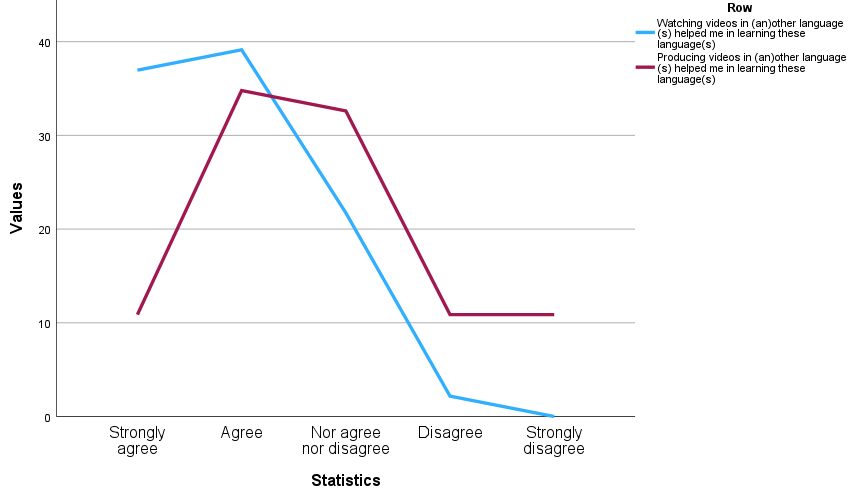
\includegraphics[width=\textwidth]{Fig-3.png}
\caption{Students' perceptions of language learning with the help
	of video watching/producing.}
\label{fig-03}
\source{Own elaboration.}
\end{minipage}
\end{figure}

It indicates that in the case of video watching, the students mostly
``strongly agree'' and ``agree'' (around 75\%) with the proposed
statement. However, in the case of video producing, most respondents
``agree'' or ``neither agree nor disagree'' (around 70\%), with some
respondents ``disagreeing'' and ``strongly disagreeing'' (around 22\%).
This comparison shows a division in opinions on the benefits of video
production, with more uncertainty in the results for video production
compared with video watching.

These results could be connected to the frequency of video production
compared to video viewing and the fact that students could be engaged in
very different forms of video production, from Instagram stories to
lengthy videos on YouTube. It can also be connected to our particular
dataset which includes students from non-language studies. In general,
we consider this discrepancy in data on video viewing and production an
interesting phenomenon for further investigation.

Additionally, we ran a cross-tabulation test with a Pearson Chi-Square
test to examine if there is a correlation between these students'
perceptions of video production (\Cref{fig-03}) and the fact that they are
current language learners (\Cref{tab-03}). The p-value (or significance) for
the Chi-Square test was 0.6, indicating no significant correlation
between these two variables. However, due to the small sample size,
seven cells had an expected count of less than 5, which may make the
results unreliable. To address this, we combined the cells ``agree'' and
``strongly agree,'' as well as ``disagree'' and ``strongly disagree,''
transforming the 5-level Likert scale into a 3-level scale. In this
adjusted analysis, only two cells had an expected count of less than 5,
making the results more reliable. Similar to the previous test, the
p-value was 0.3, indicating no significant correlation between these
categories. In addition, we ran the Fisher Exact test which is better
suited for smaller samples, nevertheless, it also did not indicate any
correlation ($p=0.7$ in the first case and $p=9.4$ in the second case).

These results indicate that there is no significant correlation between
these two categories. We also examined the categories of current
language learners and students\textquotesingle{} perceptions of video
watching, and similarly found no correlation (Chi-Square test, $p=0.5$;
Fisher Exact test, $p=0.7$). However, it would be beneficial to test this
hypothesis with a larger dataset to confirm these findings.

Moreover, we examined the relationship between the category of students'
perceptions of video production benefits and the departments where the
students study. We combined our categories into 1) Language Department,
2) Education and Psychology, and 3) Other to see if there are some
correlations between our specific dataset and the question. The
Chi-Square test showed no significant correlation $(p= 0.066)$, however,
the Fisher Exact test showed some significance $(p = 0.05)$. In this case,
as our dataset is small and 50\% of the results have an expected count
of less than 5, the Fisher Exact Test seems to be more reliable \cite{jung2014}.
\Cref{fig-04} also shows a strong indication of dependence between
these categories.

\begin{figure}[htbp]
\centering
\begin{minipage}{\textwidth}
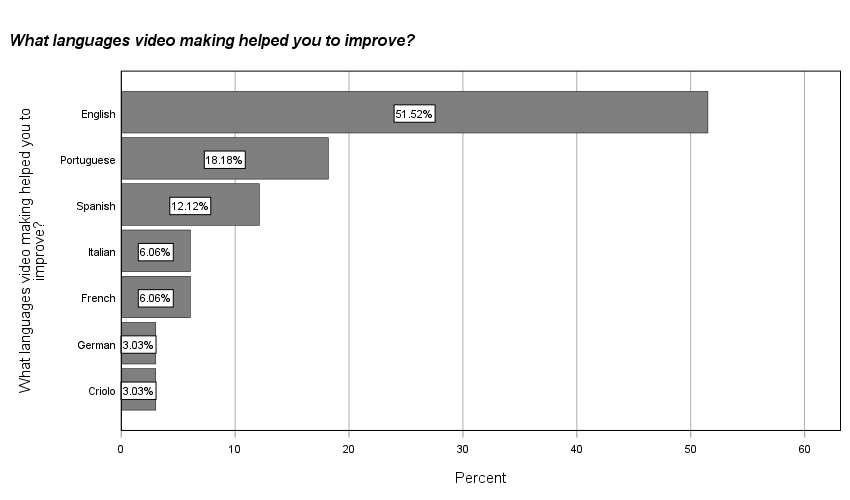
\includegraphics[width=\textwidth]{Fig-4.png}
\caption{Perceptions of the students on video production:
	department distribution.}
\label{fig-04}
\source{Own elaboration.}
\end{minipage}
\end{figure}

According to \Cref{fig-04}, we can see that in the Languages and Cultures
department, most students agree that video production helps in learning
a language (adjusted residual 1.6), while in Other Departments fewer
people agree with this statement (adjusted residual -2.5). In the
Department of Education and Psychology, fewer students disagreed that
video production could help language learning (adjusted residual -1.8).
The distribution observed here indicates more positive perceptions of
video production in the Department of Languages and Cultures. This
suggests that teaching methodologies in the Languages and Cultures and
the Education and Psychology departments may be influencing
students\textquotesingle{} perceptions. Additionally, when we tested the
correlation between a departmental distribution and students'
perceptions of video watching, we found no significant correlation using
either the Chi-Square test $(p=0.3)$ or the Fisher Exact test $(p=0.3)$.
Examining this question across different departments would be
beneficial, as our current dataset is too small to draw definitive
conclusions.

Moreover, 46\% of students chose the categories ``strongly agree'' and
``agree'' with the benefits of video production for language learning.
They also answered the next question regarding the languages that
video-making helped them learn (\Cref{tab-05}).

\begin{figure}[htbp]
\centering
\begin{minipage}{\textwidth}
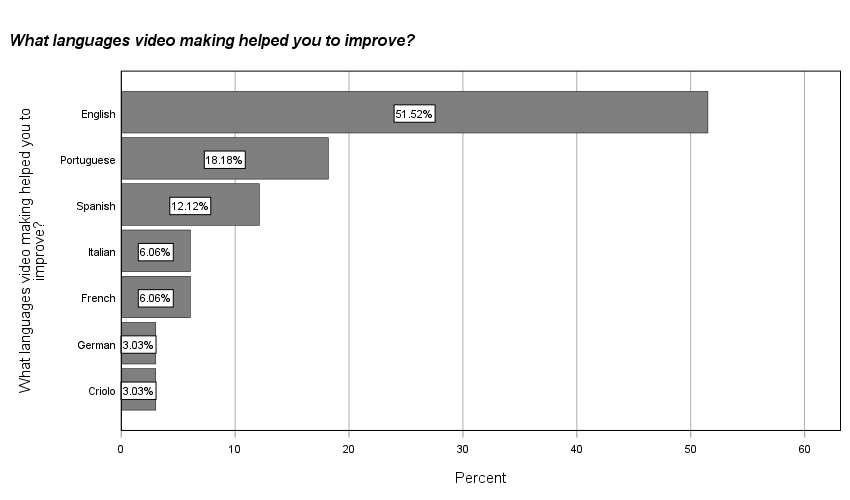
\includegraphics[width=\textwidth]{Fig-5.png}
\caption{Languages improved by making videos}
\label{fig-05}
\source{Own elaboration.}
\end{minipage}
\end{figure}

According to \Cref{fig-05}, the respondents chose a considerable variety of
languages, taking into account that only 21 people (from 46) responded
to that question and chose seven languages. English was the most popular
response, followed by Portuguese and Spanish. Notably, we can also see
\emph{Crioulo} derived from the Portuguese language (variation from Cabo
Verde) in the responses, which was completely absent from video viewing
responses \cite{shafirova2023}.

The students also responded to an open question concerning language
learning and video viewing/production: ``How have you improved your
language and cultural skills by watching/producing videos in different
languages?'' In the case of video viewing, we received 52 responses or
around 25\% of 212 respondents. According to our codebook (\Cref{annex-a}), 23
responses included the learning of vocabulary, oral comprehension had 9
responses, and pronunciation had 7. Students also noticed learning the
cultural aspects (7) of countries where languages are used and
underlined the importance of learning the language in the context of its
use (5). Overall, the detailed responses indicate that students view
this knowledge as important to share.

In the case of video production, we received 8 responses out of 46, in
other words, 17\% of the students responded, including such categories
as vocabulary (4), speaking (2) and cultural aspects (1). The answers
were less detailed than those in the viewing section, with a lower
overall response rate. Additionally, most responses came from the
Departments of Languages and Cultures and Education and Psychology. Some
responses highlighted that not only video production was beneficial for
language learning but also the work completed beforehand or afterwards
(\Cref{annex-a}). For instance, one respondent noticed: ``The research required
to produce most of my content has allowed me to widen my vision of the
English language and culture''.

We observe that students frequently highlighted vocabulary as the
primary area of improvement in both video viewing and production. This
suggests that, from the respondents\textquotesingle{} perspective,
vocabulary could be the most beneficial aspect of both practices.
